\section{Розкладання рядків (Регулярні вирази)}

\subsection{Мета:}
ознайомитися з поняттям “регулярних виразів”, синтаксисом їхнього запису та можливостями їх реалізації засобами Java; навчитись практично використовувати “регулярні вирази” для пошуку і перевірки рядків на відповідність певному шаблону.

\subsection{Теоретичний матеріал}

\begin{enumerate}
	\item Що таке “Регулярні вирази”?
	\item Засади синтаксису.
	\item Символьні класи (набір символів).
	\item Діапазони.
	\item Квантифікатори (вказівка кількості повторень).
	\item Групування.
\end{enumerate}

\subsection{Проект «Телефонний довідник»}

Програма “Телефонний довідник” імітує роботу телефонної книги та містить інформацію про абонента, номер телефону та його електронну адресу. 

\begin{figure}[h]
	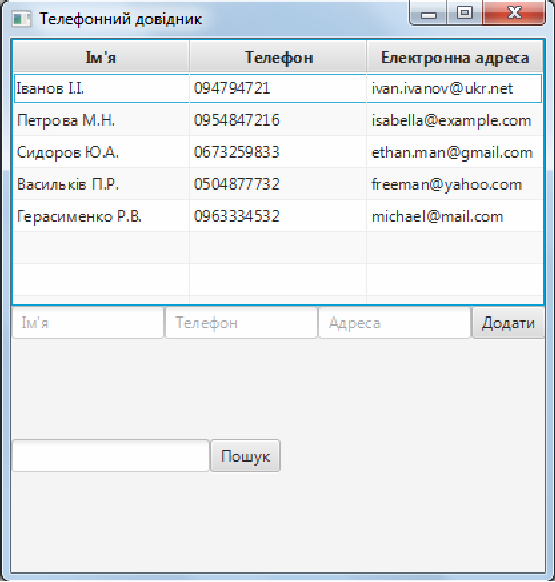
\includegraphics{javafx/images/image1.png}
	\caption{}
	\label{fig16:image1}
\end{figure}

\paragraph{Завдання:}
\begin{itemize}
	\item Створення графічного інтерфейсу для введення та виведення інформації (Рис.~\ref{fig16:image1}).
	\item Створення класу Phone для визначення абонентів  в телефонній книзі.
	\item Накладання умов на правильність занесення даних до книги.
\end{itemize}

\begin{figure}[h]
	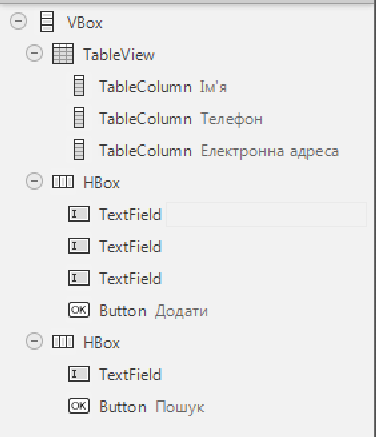
\includegraphics{javafx/images/image2.png}
	\caption{}
	\label{fig16:image2}
\end{figure}

\paragraph{Хід роботи:}
\begin{enumerate}

	\item Використовуючи Scene Builder, розробляємо інтерфейс вікна програми (Рис.~\ref{fig16:image1}). Ієрархія елементів вікна представлена на Рис.~\ref{fig16:image2}.
	\item Для створення розмітки використовуємо контейнери VBox і HBox. Для представлення даних у вигляді таблиці будемо використовувати TableView.
	\item Для елементів головного вікна програми, до яких необхідно отримати доступ з Java-коду встановлюємо fx:id:
	\begin{itemize}
		\item phoneList – таблиця для виведення інформації
		\item nameCol – поле для виведення імені
		\item phoneCol – поле для виведення номеру телефону
		\item addressCol – поле для виведення електронної адреси
		\item nameInput – поле для введення імені
		\item phoneInput – поле для введення номеру телефону
		\item addressInput – поле для введення електронної адреси
		\item addPhone – On Action для додавання абонента
		\item filterInput – поле для введення ключових значень для пошуку
		\item filterPhones – On Action для пошуку по ключовим значенням
	\end{itemize}
	\item Створюємо клас Phone, який визначає модель даних і надає методи та поля для подальшої роботи з таблицею.
\begin{minted}{java}
public class Phone {
	private final SimpleStringProperty name;
	private final SimpleStringProperty phone;
	private final SimpleStringProperty address;
	
	Phone(String name, String phone, String address) {
		this.name = new SimpleStringProperty(name);
		this.phone = new SimpleStringProperty(phone);
		this.address = new SimpleStringProperty(address);
	}
	public String getName() {
		return name.get();
	}
	public void setName(String name) {
		this.name.set(name);
	}
	public String getPhone() {
		return phone.get();
	}
	public void setPhone(String phone) {
		this.phone.set(phone);
	}
	public String getAddress() {
		return address.get();
	}
	public void setAddress(String address) {
		this.address.set(address);
	}
\end{minted}
	Об’єкти name, phone, address створені для ввімкнення посилання на певний елемент даних таблиці. Крім того, для кожного елемента даних передбачені get та set методи .
	\item В класі PhoneBookController створюємо масив ObservableList і заносимо дані про абонентів. Ці персони будуть зразу відображатись у нашій телефонній книзі. Інших абонентів можна буде додати пізніше за допомогою відповідних полів та кнопок.
\begin{minted}{java}		
	public class PhoneBookController {
		private final ObservableList<Phone> data = FXCollections.observableArrayList(
		new Phone("Іванов І.І.", "094794721", "ivan.ivanov@ukr.net"),
		new Phone("Петрова М.Н.", "0954847216", "isabella@example.com"),
		new Phone("Сидоров Ю.А.", "0673259833", "ethan.man@gmail.com"),
		new Phone("Васильків П.Р.", "0504877732", "freeman@yahoo.com"),
		new Phone("Герасименко Р.В.", "0963334532", "michael@mail.com")
		);
\end{minted}
	\item Наступним кроком є зв’язування даних зі стовпцями таблиці:
\begin{minted}{java}
@FXML public void initialize() {
	nameCol.setCellValueFactory(
	new PropertyValueFactory<Phone,String>("name")
	);
	nameCol.setCellFactory(TextFieldTableCell.forTableColumn());
	
	phoneCol.setCellValueFactory(
	new PropertyValueFactory<Phone,String>("phone")
	);
	phoneCol.setCellFactory(TextFieldTableCell.forTableColumn());
	
	addressCol.setCellValueFactory(
	new PropertyValueFactory<Phone,String>("address")
	);
	addressCol.setCellFactory(TextFieldTableCell.forTableColumn());
	nameCol.setOnEditCommit(
	new EventHandler<CellEditEvent<Phone, String>>() {
		@Override
		public void handle(CellEditEvent<Phone, String> t) {
			Pattern ptNameColl = Pattern.compile("[A-ZА-ЯІ]{1}[a-zа-яі]+\\s[A-ZА-ЯІ]{1}\\.[A-ZА-ЯІ]{1}\\.");
			Matcher n = ptNameColl.matcher(t.getNewValue());
			boolean fpn = n.matches();
			if (fpn) {
				((Phone) t.getTableView().getItems().get(
				t.getTablePosition().getRow())
				).setName(t.getNewValue());
				
			}
			phoneList.refresh();
		}
	}
	);
	phoneCol.setOnEditCommit(
	new EventHandler<CellEditEvent<Phone, String>>() {
		
		@Override
		public void handle(CellEditEvent<Phone, String> t) {
			Pattern ptPhoneColl = Pattern.compile("[0-9]+");
			Matcher p = ptPhoneColl.matcher(t.getNewValue());
			boolean fpp = p.matches();
			if (fpp) {
				((Phone) t.getTableView().getItems().get(
				t.getTablePosition().getRow())
				).setPhone(t.getNewValue());
			}
			phoneList.refresh();
		}
	}
	
	
	);
	addressCol.setOnEditCommit(
	new EventHandler<CellEditEvent<Phone, String>>() {
		@Override
		public void handle(CellEditEvent<Phone, String> t) {
			Pattern ptAddressColl = Pattern.compile("[a-z0-9]{1,}@{1}([a-z0-9]{1,}\\.)+[a-z]{1,3}");
			Matcher a = ptAddressColl.matcher(t.getNewValue());
			boolean fpa = a.matches();
			if (fpa) {
				((Phone) t.getTableView().getItems().get(
				t.getTablePosition().getRow())
				).setAddress(t.getNewValue());
			}
			phoneList.refresh();
		}
	}
	);
	
	phoneList.setItems(filteredData);
	
}
\end{minted}
	\item Наступна частина коду дозволяє перевіряти на валідність введення даних до телефонної книги, яку ми записуємо в класі Phone:
\begin{minted}{java}
public boolean isValidName() {
	Pattern ptN = Pattern.compile("[A-ZА-ЯІ]{1}[a-zа-яі]+\\s[A-ZА-ЯІ]{1}\\.[A-ZА-ЯІ]{1}\\.");
	Matcher n = ptN.matcher(getName());
	boolean fn = n.matches();
	return fn;
}
public boolean isValidPhone() {
	Pattern ptP = Pattern.compile("[0-9]+");
	Matcher p = ptP.matcher(getPhone());
	boolean fp = p.matches();
	return fp;
}
public boolean isValidAddress() {
	Pattern ptA = Pattern.compile("[a-z0-9]{1,}@{1}([a-z0-9]{1,}\\.)+[a-z]{1,3}");
	Matcher a = ptA.matcher(getAddress());
	boolean fa = a.matches();
	return fa;
}
\end{minted}
		Можна побачити, що для перевірки правильності введення даних ми використовуємо регулярні вирази (пишемо символьні класи, вказуємо діапазони та кількість повторень) для імені, номеру телефону та електронної адреси.
	\item Для додавання нових абонентів в PhoneBookController створюємо обробник події для кнопки addPhone:
\begin{minted}{java}
@FXML public void addPhone() {
	Phone p = new Phone(nameInput.getText(), phoneInput.getText(), addressInput.getText());
	if ((p.isValidName())&&(p.isValidPhone())&&(p.isValidAddress())) {
		data.add(p);
		nameInput.clear();
		phoneInput.clear();
		addressInput.clear();
	}
	if (p.isValidName()==false){
		nameInput.setStyle("-fx-text-fill: red");
	}else {
		nameInput.setStyle("-fx-text-fill: black");
	}
	if (p.isValidPhone()==false){
		phoneInput.setStyle("-fx-text-fill: red");
	}else {
		phoneInput.setStyle("-fx-text-fill: black");
	}
	if (p.isValidAddress()==false){
		addressInput.setStyle("-fx-text-fill: red");
	}else {
		addressInput.setStyle("-fx-text-fill: black");
	}
}
\end{minted}
		Тут передбачено забарвлення тексту в червоний колір, якщо дані, які вводяться, неправильні або не відповідають шаблону введення (прикладом може бути букви в номері телефону чи неправильний e-mail).
	\item Для пошуку даних в класі PhoneBookController створюємо обробник події для кнопки filterPhones:
\begin{minted}{java}
	@FXML public void filterPhones() {
		filteredData.setPredicate(e -> e.getName().contains(filterInput.getText()));
	}
	private final FilteredList<Phone> filteredData = new FilteredList<>(data, p -> true);
}
\end{minted}
	\item Для редагування елементів в таблиці використовуємо метод setOnEditCommit, який зазначений в п.6. При редагуванні ми також перевіряємо дані на правильність введення, використовуючи регулярні вирази.
\begin{minted}{java}
nameCol.setOnEditCommit(
new EventHandler<CellEditEvent<Phone, String>>() {
	@Override
	public void handle(CellEditEvent<Phone, String> t) {
		Pattern ptNameColl = Pattern.compile("[A-ZА-ЯІ]{1}[a-zа-яі]+\\s[A-ZА-ЯІ]{1}\\.[A-ZА-ЯІ]{1}\\.");
		Matcher n = ptNameColl.matcher(t.getNewValue());
		boolean fpn = n.matches();
		if (fpn) {
			((Phone) t.getTableView().getItems().get(
			t.getTablePosition().getRow())
			).setName(t.getNewValue());
			
		}
		phoneList.refresh();
	}
}
);

phoneCol.setOnEditCommit(
new EventHandler<CellEditEvent<Phone, String>>() {
	
	@Override
	public void handle(CellEditEvent<Phone, String> t) {
		Pattern ptPhoneColl = Pattern.compile("[0-9]+");
		Matcher p = ptPhoneColl.matcher(t.getNewValue());
		boolean fpp = p.matches();
		if (fpp) {
			((Phone) t.getTableView().getItems().get(
			t.getTablePosition().getRow())
			).setPhone(t.getNewValue());
		}
		phoneList.refresh();
	}
}


);

addressCol.setOnEditCommit(
new EventHandler<CellEditEvent<Phone, String>>() {
	@Override
	public void handle(CellEditEvent<Phone, String> t) {
		Pattern ptAddressColl = Pattern.compile("[a-z0-9]{1,}@{1}([a-z0-9]{1,}\\.)+[a-z]{1,3}");
		Matcher a = ptAddressColl.matcher(t.getNewValue());
		boolean fpa = a.matches();
		if (fpa) {
			((Phone) t.getTableView().getItems().get(
			t.getTablePosition().getRow())
			).setAddress(t.getNewValue());
		}
		phoneList.refresh();
	}
}
);
\end{minted}
	\item Клас Main:
\begin{minted}{java}
public class Main extends Application {
	@Override
	public void start(Stage primaryStage) {
		try {
			VBox root = (VBox)FXMLLoader.load(getClass().getResource("PhoneBook.fxml"));
			Scene scene = new Scene(root,400,400);
			scene.getStylesheets().add(getClass().getResource("application.css").toExternalForm());
			primaryStage.setTitle("Телефонний довідник");
			primaryStage.setScene(scene);
			primaryStage.show();
		} catch(Exception e) {
			e.printStackTrace();
		}
	}
	
	public static void main(String[] args) {
		launch(args);
	}
}
\end{minted}
	
\end{enumerate}

\subsection{Задачі для самостійного виконання}
В даному проекті створіть можливість передбачення уведення телефонного номера у форматі (ххх)-ххх-хх-хх.